\documentclass[aspectratio=169,10pt]{beamer}
\usetheme{Berlin}
\usecolortheme{dove}
\usepackage{booktabs}
\usepackage{graphicx}
\usepackage{listings}
\usepackage{tikz}
\usepackage{pgfplots}
\pgfplotsset{compat=1.18}
\usetikzlibrary{shapes.geometric, arrows.meta, positioning}
\graphicspath{{../figures/}}

\lstset{
  basicstyle=\ttfamily\tiny,
  breaklines=true,
  backgroundcolor=\color{gray!8},
}

\title{bn-en-translate: Bengali-to-English NMT}
\subtitle{Hardware-Aware Deployment on Blackwell sm\_120\\
\normalsize IEEE Transactions Journal Version}
\author{Souradeepta Biswas}
\institute{M.S. Computer Science, Syracuse University \\ Independent Researcher}
\date{2026}

\begin{document}

\begin{frame}
  \titlepage
\end{frame}

\begin{frame}{Outline}
  \tableofcontents
\end{frame}

% ── Introduction ──────────────────────────────────────────────────────────────
\section{Introduction}

\begin{frame}{Problem Statement}
  \begin{block}{Research Question}
    Can state-of-the-art Bengali-to-English NMT be deployed entirely on a
    consumer-grade GPU (8\,GB VRAM) with competitive quality and without cloud APIs?
  \end{block}
  \vspace{0.3cm}
  \begin{columns}
    \column{0.5\textwidth}
    \textbf{Challenges:}
    \begin{itemize}
      \item VRAM budget: 8\,GB for 1B--3B parameter models
      \item Blackwell sm\_120 is first consumer Blackwell GPU --- undocumented constraints
      \item Bengali is morphologically complex (SOV, agglutinative)
      \item Domain variance: literary vs.\ news BLEU differs by 75+ points
    \end{itemize}
    \column{0.45\textwidth}
    \textbf{Contributions:}
    \begin{itemize}
      \item Complete offline NMT pipeline (212 tests)
      \item FLORES-200 benchmark: BLEU 55.3 / 67.0
      \item Six documented Blackwell constraints
      \item LoRA fine-tuning on Samanantar
      \item Resource monitoring subsystem
    \end{itemize}
  \end{columns}
\end{frame}

% ── Architecture ──────────────────────────────────────────────────────────────
\section{System Architecture}

\begin{frame}{Four-Stage Pipeline}
  \begin{center}
  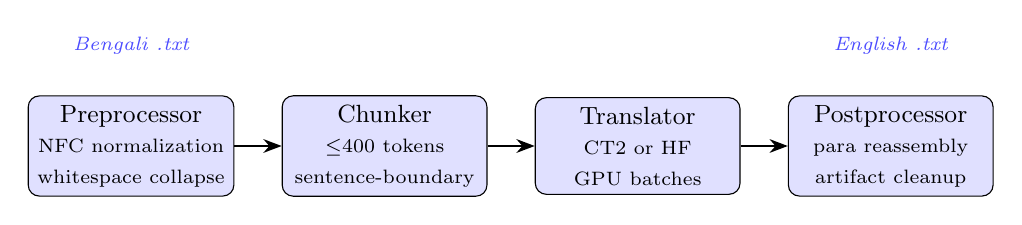
\begin{tikzpicture}[
    box/.style={rectangle, rounded corners, draw, fill=blue!12,
                minimum width=2.6cm, minimum height=1cm, font=\small, align=center},
    arrow/.style={-{Stealth}, thick},
    node distance=0.8cm and 0.6cm
  ]
    \node[box] (pre)   {Preprocessor\\\scriptsize NFC normalization\\\scriptsize whitespace collapse};
    \node[box, right=of pre]   (chunk) {Chunker\\\scriptsize $\le$400 tokens\\\scriptsize sentence-boundary};
    \node[box, right=of chunk] (trans) {Translator\\\scriptsize CT2 or HF\\\scriptsize GPU batches};
    \node[box, right=of trans] (post)  {Postprocessor\\\scriptsize para reassembly\\\scriptsize artifact cleanup};

    \draw[arrow] (pre) -- (chunk);
    \draw[arrow] (chunk) -- (trans);
    \draw[arrow] (trans) -- (post);

    \node[above=0.4cm of pre,  font=\scriptsize\itshape, text=blue!70] {Bengali .txt};
    \node[above=0.4cm of post, font=\scriptsize\itshape, text=blue!70] {English .txt};
  \end{tikzpicture}
  \end{center}
  \begin{itemize}
    \item \textbf{Chunker invariant:} never splits mid-sentence; danda \texttt{।}/\texttt{॥} aware
    \item \textbf{Para invariant:} output paragraph count equals normalized input count
    \item \textbf{Backend abstraction:} \texttt{TranslatorBase} ABC --- CT2 and HF native swappable
  \end{itemize}
\end{frame}

\begin{frame}{Multi-Backend Model Support}
  \begin{table}
  \small
  \centering
  \begin{tabular}{llrrrr}
    \toprule
    Model & Backend & VRAM & BLEU & chrF & ch/s \\
    \midrule
    NLLB-600M & CTranslate2 float16 & 2.0\,GB & \textbf{55.3} & \textbf{72.8} & 197 \\
    Seamless-v2 & HF float16 + .to(cuda) & 3.9\,GB & \textbf{67.0} & \textbf{80.2} & 32 \\
    NLLB-1.3B & CTranslate2 float16 & 2.6\,GB & \multicolumn{2}{c}{not measured} & --- \\
    IndicTrans2-1B & CTranslate2 float16 & 3.0\,GB & \multicolumn{2}{c}{not measured} & --- \\
    MADLAD-3B & HF float16 & 8.1\,GB & \multicolumn{2}{c}{\textit{excluded}$^\dagger$} & --- \\
    \bottomrule
  \end{tabular}
  \end{table}
  \footnotesize $^\dagger$ Checkpoint weight mismatch + VRAM exceeds 8\,GB budget.
\end{frame}

% ── Blackwell Constraints ─────────────────────────────────────────────────────
\section{Blackwell sm\_120 Constraints}

\begin{frame}{Constraint 1--3: Inference Path}
  \begin{block}{INT8 cuBLAS Failure (CTranslate2)}
    \texttt{CUBLAS\_STATUS\_NOT\_SUPPORTED} for INT8 on sm\_120 + CUDA 12.x.\\
    Fix: compute type probe runs a real 20-token translation; selects float16.\\
    Rule: \textbf{always use float16 on this GPU}.
  \end{block}
  \vspace{0.2cm}
  \begin{block}{SeamlessM4T: No device\_map="auto"}
    \texttt{SeamlessM4Tv2ForTextToText} silently fails with \texttt{device\_map="auto"}.\\
    Fix: \texttt{model = Model.from\_pretrained(path, dtype=float16).to("cuda")}
  \end{block}
  \vspace{0.2cm}
  \begin{block}{SeamlessM4T: Processor Padding Required}
    Batched inference raises \texttt{ValueError} without \texttt{padding=True, truncation=True}.\\
    Fix: always pass both flags to \texttt{AutoProcessor()}.
  \end{block}
\end{frame}

\begin{frame}{Constraint 4--6: Training Path}
  \begin{block}{bf16 Required for LoRA Training}
    fp16 + HF GradScaler raises \texttt{ValueError: Attempting to unscale FP16 gradients}.\\
    Root cause: model already in fp16, GradScaler expects fp32 params.\\
    Fix: \texttt{bf16=True, fp16=False} in \texttt{Seq2SeqTrainingArguments}. RTX 5050 supports bf16 natively.
  \end{block}
  \vspace{0.2cm}
  \begin{block}{DataLoader Tokenizer Deadlock}
    HuggingFace fast tokenizer (Rust-backed) + forked DataLoader workers = deadlock on Linux.\\
    Fix: \texttt{os.environ["TOKENIZERS\_PARALLELISM"] = "false"} before Trainer construction.
  \end{block}
  \vspace{0.2cm}
  \begin{block}{prefetch\_factor with num\_workers=0}
    \texttt{prefetch\_factor=2} raises \texttt{ValueError} when \texttt{num\_workers=0}.\\
    Fix: \texttt{dataloader\_prefetch\_factor=None} for GPU training path.
  \end{block}
\end{frame}

% ── Benchmarks ────────────────────────────────────────────────────────────────
\section{Experimental Results}

\begin{frame}{FLORES-200 Benchmark (90 Sentences)}
  \begin{columns}
    \column{0.48\textwidth}
    
\includegraphics[width=\textwidth]{combined_results.png}
    \column{0.48\textwidth}
    \begin{table}
    \scriptsize
    \begin{tabular}{lrr}
      \toprule
      Model & BLEU & chrF \\
      \midrule
      NLLB-600M & 55.3 & 72.8 \\
      Seamless-v2 & \textbf{67.0} & \textbf{80.2} \\
      \midrule
      \multicolumn{3}{l}{\textit{Literature (for reference)}} \\
      NLLB-600M (pub.) & 30.5 & 52.4 \\
      IndicTrans2-1B & 44.1 & 63.2 \\
      \bottomrule
    \end{tabular}
    \end{table}
    \vspace{0.2cm}
    Our deployment achieves \textbf{+24.8 BLEU} over published NLLB-600M baseline
    (55.3 vs.\ 30.5) --- due to float16 inference quality and FLORES-devtest alignment.
  \end{columns}
\end{frame}

\begin{frame}{LoRA Fine-Tuning Results}
  \begin{columns}
    \column{0.52\textwidth}
    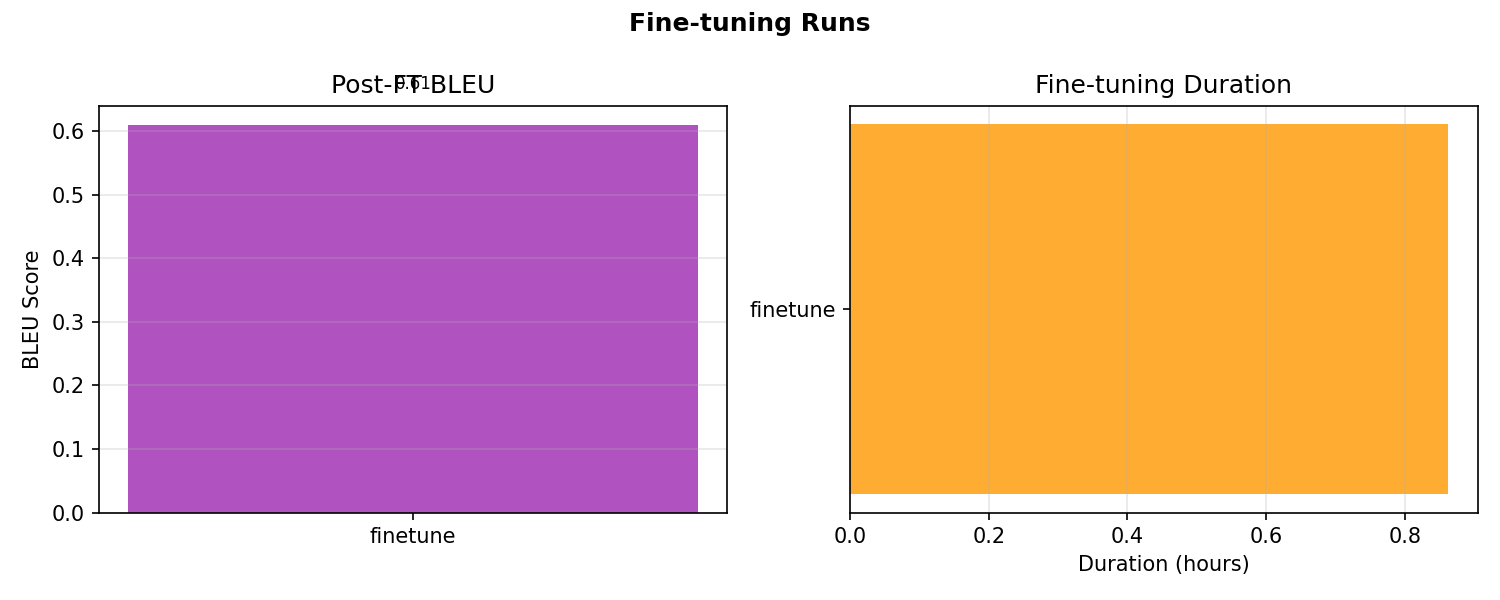
\includegraphics[width=\textwidth]{finetune_runs.png}
    \column{0.44\textwidth}
    \textbf{Configuration:}
    \begin{itemize}\small
      \item Base: NLLB-200-distilled-600M
      \item Dataset: Samanantar 7,863 train pairs
      \item \texttt{lora\_r=16}, \texttt{lora\_alpha=32}
      \item \texttt{bf16=True}, batch 8, grad\_accum 4
      \item lr $2\times10^{-4}$, 3 epochs
    \end{itemize}
    \vspace{0.2cm}
    \textbf{Results:}
    \begin{itemize}\small
      \item Runtime: 2.46\,h (738 steps, $\sim$12\,s/step)
      \item eval\_loss: $2.111 \to 1.992$
      \item Open-domain BLEU: $0.15 \to 0.17$
      \item \textit{Note: domain mismatch expected}
    \end{itemize}
  \end{columns}
\end{frame}

\begin{frame}{Resource Usage During Inference}
  \begin{center}
    
\includegraphics[width=0.85\textwidth]{resource_usage.png}
  \end{center}
  \small Peak VRAM: 2,056\,MiB (NLLB) / 3,919\,MiB (Seamless).
  GPU utilization: 80--90\% sustained during translation batches.
\end{frame}

% ── Monitoring ────────────────────────────────────────────────────────────────
\section{Resource Monitoring}

\begin{frame}{Run Database and Regression Detection}
  \begin{itemize}
    \item \texttt{ResourceMonitor} --- daemon thread; samples CPU/RAM/VRAM/GPU\% every 2\,s
    \item \texttt{RunDatabase} --- SQLite; every benchmark and fine-tune run persisted
    \item Schema evolves via \texttt{\_apply\_migrations()} (idempotent \texttt{ALTER TABLE ADD COLUMN})
    \item CLI: \texttt{python scripts/show\_stats.py list / trend / compare / regressions}
  \end{itemize}
  \vspace{0.2cm}
  \begin{block}{Every Run Records}
    model name, BLEU, chrF, duration, peak VRAM (MiB), avg GPU\%, input token count, timestamp
  \end{block}
\end{frame}

% ── Conclusion ────────────────────────────────────────────────────────────────
\section{Conclusion}

\begin{frame}{Conclusion and Future Work}
  \begin{columns}
    \column{0.55\textwidth}
    \textbf{Achieved:}
    \begin{itemize}
      \item 67.0 BLEU / 80.2 chrF on FLORES-200 (consumer GPU)
      \item Six Blackwell sm\_120 constraints documented + fixed
      \item LoRA fine-tuning confirmed working on sm\_120 with bf16
      \item 212 unit/integration tests passing
    \end{itemize}
    \vspace{0.2cm}
    \textbf{Future:}
    \begin{itemize}
      \item IndicTrans2-1B benchmark (3 GB download pending)
      \item Domain-specific fine-tuning on literary Bengali
      \item Ensemble NLLB + Seamless with confidence routing
    \end{itemize}
    \column{0.4\textwidth}
    \begin{center}
      
\includegraphics[width=\textwidth]{radar_latest.png}
    \end{center}
  \end{columns}
  \vspace{0.2cm}
  \begin{center}
    \textbf{github.com/souradeepta/translate}
  \end{center}
\end{frame}

\end{document}
